%  --------------------------------------------------------------------------
%  IPA Qualitätssicherung für Djangoprojekte Dokumentation
%  Created by Vladimir Kuzma on 2012-04-30.
%  --------------------------------------------------------------------------

%  --------------------------------------------------------------------------
%  Latex Document Settings
%  --------------------------------------------------------------------------

\documentclass[
11pt, % Schriftgrösse
a4paper, % A4 Papier
BCOR10mm, % Absoluter Wert der Bindekorrektur, z.B. BCOR1cm
DIV14, % Satzspiegel festlegen siehe
       % http://www.ctex.org/documents/packages/nonstd/koma-script.pdf
footsepline = false, % Trennlinie zwischen Textkörper und Fußzeile
                     % bei normalen Seiten
headsepline, % Trennlinie zwischen Kopfzeile und Textkörper
             % bei normalen Seiten
oneside, % Zweiseitig
openright,
halfparskip, % Europäischer Satz mit Abstand zwischen den Absätzen
abstracton, % inkl. Abstract
listof=totocnumbered, % Abb.- und Tab.verzeichnis im Inhaltsverzeichnis
bibliography=totocnumbered % Lit.zeichnis in Inhaltsverzeichnis aufnehmen
]{scrreprt}

\usepackage[automark]{scrpage2} % Gestaltung von kopf- und Fußzeile
\usepackage[ngerman]{babel}
\usepackage[ngerman]{translator}
\usepackage{tocbasic}
\usepackage[utf8]{inputenc}
\usepackage{lmodern} % Latin Modern
\usepackage[T1]{fontenc}
\usepackage{hyphenat}
\usepackage{ae} % Schöne Schriften für PDF-Dateien

% Tradmark
\def\TTra{\textsuperscript{\texttrademark}}

%1.5 Zeilenabstand
\usepackage[onehalfspacing]{setspace}

% Festlegung des Seitenstils (scrpage2)
\pagestyle{scrheadings}
\clearscrheadfoot
\automark[chapter]{section}

% \lehead{\sffamily\upshape\headmark}
% \cehead{}
% \rehead{}
% \lefoot[\pagemark]{\upshape \pagemark}
% \cefoot{}
% \refoot{}
% \lohead{}
% \cohead{}
\lohead{\sffamily\upshape\headmark}
\lofoot{}
\cofoot[\today]{\today}
\rofoot[\pagemark]{\scshape \pagemark}

% Surround parts of graphics with box
\usepackage{boxedminipage}

% Package for including code in the document
\usepackage{listings}

% If you want to generate a toc for each chapter (use with book)
\usepackage{minitoc}
\usepackage{longtable}

% Abkürzungsverzeichnis erstellen.
\usepackage[printonlyused]{acronym}

% schöne Tabelle zeichnen
\usepackage{booktabs}
\renewcommand{\arraystretch}{1.4} %Die Zeilenabstände in Tabellen angepasst.

% für variable Breiten
\usepackage{tabularx}

% Durchgestrichener Text
\usepackage[normalem]{ulem} %emphasize weiterhin kursiv

% This is now the recommended way for checking for PDFLaTeX:
\usepackage{ifpdf}

\usepackage{eurosym}

\usepackage{natbib}

\usepackage{paralist}

\usepackage{array,ragged2e}

\usepackage[hyperfootnotes=false]{hyperref}
\hypersetup{
  bookmarks=true,         % show bookmarks bar?
  unicode=true,           % non-Latin characters in Acrobat’s bookmarks
  pdftoolbar=true,        % show Acrobat’s toolbar?
  pdfmenubar=true,        % show Acrobat’s menu?
  pdffitwindow=true,      % window fit to page when opened
  pdfstartview={FitH},    % fits the width of the page to the window
  pdftitle={IPA Dokumentation},   
  pdfauthor={Marius Küng},
  pdfsubject={Dokumentation IPA yatplaner},
  pdfcreator={TeX Live 2009},
  pdfproducer={pdfTeX, Version 3.1415926-1.40.10},
  pdfnewwindow=true,      % links in new window
  colorlinks=true,       % false: boxed links; true: colored links
  linkcolor=black,          % color of internal links
  citecolor=black,        % color of links to bibliography
  filecolor=magenta,      % color of file links
  urlcolor=cyan          % color of external links
  % linkcolor=black,          % color of internal links
  % citecolor=black,        % color of links to bibliography
  % filecolor=black,      % color of file links
  % urlcolor=black          % color of external links
}

\ifpdf
    \usepackage[pdftex]{graphicx}
\else
    \usepackage{graphicx}
\fi

\makeatletter 
\let\orgdescriptionlabel\descriptionlabel 
\renewcommand*{\descriptionlabel}[1]{% 
  \let\orglabel\label 
  \let\label\@gobble 
  \phantomsection 
  \edef\@currentlabel{#1}% 
  %\edef\@currentlabelname{#1}% 
  \let\label\orglabel 
  \orgdescriptionlabel{#1}% 
} 
\makeatother 

%  --------------------------------------------------------------------------
%  Start Document
%  --------------------------------------------------------------------------
\title{Dokumentation IPA Qualitätssicherung für Djangoprojekte}

\author{IPA in Applikationsentwicklung\\
    \\
    Auszubildender - Vladimir Kuzma\\
	Auftraggeber - allink GmbH\\
    Projektleiter - Silvan Spross\\
    Experte - Roman Fischer\\
    Chefexperte -  \\
    Durchführungsort - allink GmbH\\
	\\
	Informatikschule ZLI }

\date{30.04. - 16.05.2012}

\begin{document}
    \ifpdf
        \DeclareGraphicsExtensions{.pdf, .jpg, .tif}
    \else
        \DeclareGraphicsExtensions{.eps, .jpg}
    \fi

    \pagenumbering{Alph}
  
    \maketitle

    \pagenumbering{arabic}
  
    \tableofcontents
    
    \part{Umfeld und Ablauf}
         \chapter{Aufgabenstellung}
             %!TEX root = ../dokumentation.tex
\section{Titel der Facharbeit} 
Kontinuierliche Qualitätssicherung für Web Projekte in Django
    
\section{Thematik}
Es soll eine Software in Python erstellt werden, welche kontinuierlich die Qualität von einer konfigurierbaren Menge Django Projekte überprüft.

\section{Klassierung}
    
\begin{itemize}
    \item Prozessautomatisierung 
    \item UNIX / Linux
    \item Python / Ruby
\end{itemize}
    
\section{Durchführungsblock}
Startblock 10: 16.04.2012 - 20.04.2012\\
IPA-Durchführung: 30.04.2012 - 16.05.2012\\
Einreichung bis: Montag, 16.03.2012\\
    
\section{Ausgangslage}
Bei allink besteht seit Mitte 2010 ein Entwicklungs- und Deployment-Prozess welcher sich in den letzten eineinhalb Jahren etabliert hat. Die Entwickler sparen sich dadurch pro Projekt einige Stunden Arbeit und die Projekte sind zudem auch nach längere Zeit noch wartbar. Dank der Abhängigkeitsdefinitionen pro Projekt, können Entwickler schnell in einem anderem Projekt einsteigen oder in einem alten Projekt Fehlerkorrekturen vornehmen. Seit einem halben Jahr wird zudem die Codequalität mit Hilfe von einer automatischen Überprüfung der Codekonvention auf den Rechnern der Entwickler erhöht.

Trotz all diesen Massnahmen ist es möglich, dass Entwickler ein Projekt unabsichtlich verunreinigen. Im Extremfall führt dies dazu, dass das Projekt bei einem anderen Entwickler oder sogar in der Produktion nicht mehr lauffähig ist.

Mit dieser Arbeit soll ein System zur automatischen Kontrolle der erwähnten Faktoren erstellt werden.

\section{Detaillierte Aufgabenstellung}
Es soll eine Software in Python erstellt werden, welche kontinuierlich die Qualität von einer konfigurierbaren Menge Django Projekte überprüft. Dazu sollen die Projekte jeweils täglich aus dem Versionierungssystem geklont, Projektspezifische Abhängigkeiten installiert und nach gewissen Anforderungen getestet und abschliessend ein projektübergreifender Report per E-Mail versendet werden.

Diese Anforderungen sind:

- Installierbarkeit der projektspezifischen Abhängigkeiten
Erklärung: Jedes Projekt hat projektspezifische Abhängigkeiten, welche sich über ein Packetmanagement installieren lassen. Bei dieser Anforderung soll pro Projekt geprüft werden, ob diese Abhängigkeitsliste komplett und korrekt ist.

- Codekonventionen nach PEP8
Erklärung: Im ''Python Enhancement Proposal 8'' sind die grundlegenden Stil-Richtlinien für Python-Quellcode definiert. Bei dieser Anforderung soll pro Projekt geprüft werden, dass diese Stil-Richtlinien eingehalten wurden.

- Überprüfung der Syntax
Erklärung: Überprüft werden sollen sämtliche Python und Javascript Files z.B. mit pyflakes und jshint.

- Initialisierung der Datenbank

- Durchführen sämtlicher Datenbankmigrations-Files

- UnitTests

Treten bei den Tests Fehler auf, soll dies in einem E-Mail festgehalten und an eine Sammeladresse gesendet werden.

Eine weitere Anforderung an die Software ist, dass die einzelnen Überprüfungen der Anforderungen Modular aufgebaut sind und so in Zukunft weitere Anforderungen hinzugefügt werden können. Zudem kommt hinzu, dass die neu zu schreibende Applikation mit dem Versionsverwaltungssystem git verwaltet werden soll. Dabei sollen zwei Branches geführt werden: ''develop'' und ''master''. Wobei der ''master'' immer den Stand der Produktion widerspiegelt und im ''develop'' weiterentwickelt wird.

Es sollen wo möglich bestehende Tools zur Überprüfung der oben genannten Anforderungen verwendet werden. Dies bedeutet für den Lernenden, dass er überwiegend die Software zum Koordinieren und zusammenführen der einzelnen Tests schreiben muss.

Nicht Bestandteil dieser Arbeit sind:

- VirtualMachine zur Entwicklung
- Bereitstellung des Zielsystems
- Einpflegen aller Projekte

Nebst der begleitenden IPA Dokumentation wird keine zusätzliche Dokumentation gefordert.

\section{Mittel und Methoden}
Folgende Technologien sind zwingend zu verwenden:

\begin{itemize}
    \item  Python 2.x
    \item  Django
\end{itemize}

Der Lernende muss sich zudem während der Entwicklung an die Firmenstandards halten, welche im IT Wiki zugänglich sind.
    
\section{Vorkenntnisse}
Dem Lernenden sind alle genannten Technologien bereits bekannt. Seit Beginn seines Praktikums im Mai 2010 setzt er sich damit auseinander.
    
\section{Vorarbeiten}
Die Testumgebung wird als VirtualMachine Image mit einem unserem Produktivsystem am nächsten kommenden System bespielt und dem Lernenden zur Verfügung gestellt.    

\section{Neue Lerninhalte}
Wie erwähnt sind dem Lernenden alle Technologien bereits bekannt. Das Know-how ist zudem bei allink ausreichend vorhanden. 

\section{Arbeiten in den letzten 6 Monaten}
Der Lernende hat diverse Webseiten mit den oben genannten Technologien umgesetzt.

        \chapter{Einleitung}
            %!TEX root = ../dokumentation.tex
\section{Projekorganisation}

\begin{figure}[!ht]
\begin{center}
    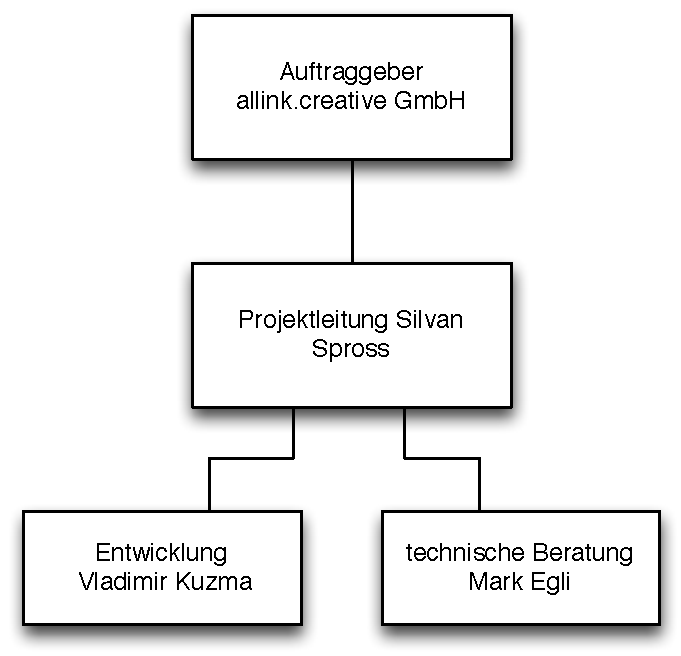
\includegraphics[width=0.5\textwidth,angle=0]{./grafiken/organigram.pdf}
\end{center}
\end{figure}
\footnotetext{Eigene Darstellung}

\section{Projektbeschreibung}
Es soll eine Software in Python erstellt werden, welche kontinuierlich die Qualität von einer konfigurierbaren Menge Django Projekte überprüft. Dazu sollen die Projekte jeweils täglich aus dem Versionierungssystem geklont, Projektspezifische Abhängigkeiten installiert und nach gewissen Anforderungen getestet und abschliessend ein projektübergreifender Report per E-Mail versendet werden.

\section{Rahmenbedingung}
Die Anwendung soll mit folgenden Mitteln realisiert werden:

Technologien
\begin{itemize}
    \item Python 

\end{itemize}

Anwendungen
\begin{itemize}
    \item pep8
    \item pyflakes
    \item jshint
\end{itemize}

Systemen
\begin{itemize}
    \item Mac OS X
    \item Debian lenny
\end{itemize}
    
\section{Systemumgebung}
\begin{itemize}
    \item Betriebsystem (Projekumsetzung): Mac OS X
    \item Editor: vim
    \item Dokumentationshilfsmittel: LaTeX
    \item Entwicklungsumgebung: Python
    \item localer Testserver: Debian Server in einer VM (Virtualbox) 
    \item Versionierung: Git, auf Github veröffentlicht
\end{itemize}

\section{Projektplannungsmethode}
Ich habe mich für die Projektplanungsmethode IPERKA entschieden. \\

\subsection{Begründung}
Für ein kleines Projekt reicht IPERKA meiner Meinung ausreichend aus. Die Planungs- und die Realisierungsphase ist klar getrennt. Es sind alle wichtigen Arbeitsschritte vorhanden, die eine saubere Struktur und ausführliche Dokumentation erlauben. 

\clearpage

         \chapter{Analyse}
            %!TEX root = ../dokumentation.tex
\section{Analyse des Ist-Zustands}
Momentan werden unsere Djangoprojekte beim Commiten (Versionierung mit Hilfen von git) mit sognenannten ''pre-commit hooks'' analysiert. 
Dabei wird der Quellcode auf diverse Aspekte überprüft. Bei nicht bestehender Überprüfung wird eine Meldung ausgegeben.\\

\begin{center}
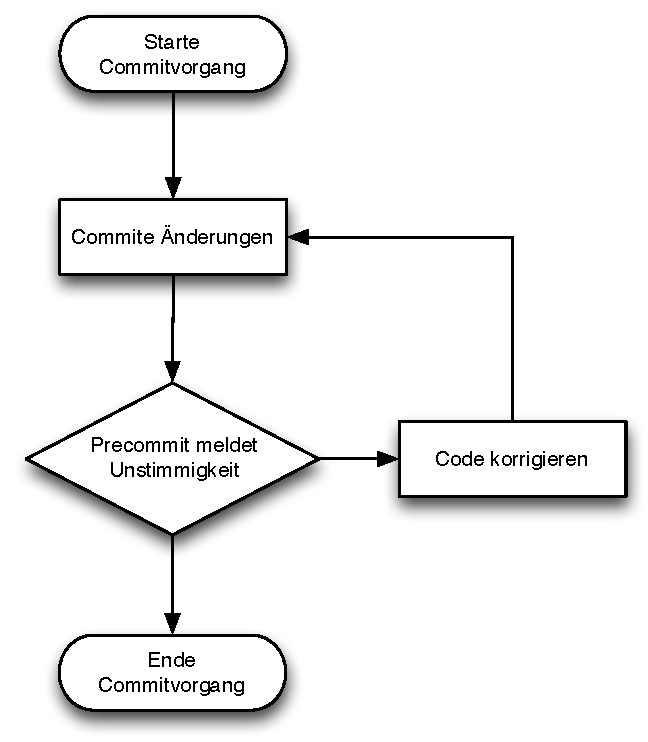
\includegraphics[width=0.6\textwidth,angle=0]{./grafiken/pzd_projektabarbeitung_ist.pdf}
\end{center}

Diese Methode hat bisher die Fehlerquate um einiges verringert. Es ist jedoch immer noch möglich einen Fehler in die Produktion einzuspielen. \\  
Folgende Ursachen können trotz pre-commit hooks einen Fehler auslösen. 
\begin{itemize}
    \item Man commited direkt über Github.
    \item Das requirements.txt für pip ist nicht vollständig.
    \item Programmierfehler, die nicht die Syntax betreffen. 
\end{itemize}
Derzeitig wird der Quellcode nach folgenden Zeichenkette überprüft:
\begin{itemize}
    \item ''import pdb'' - *.py: 
        pdb ist der Python Debugger. Aus Sicherheitsgründen darf dieser nicht in der Produktion verwendet werden.
    \item ''import ipdb'' - *.py:
        Gleiche Begründung wie ''import pdb''.
    \item ''print'' - *.py:
        Konsolenausgabe sind in der Produktion unerwünscht.
    \item ''console.log'' - *.js:
        Konsolenausgabe sind in der Produktion unerwünscht.
    \item ''debugger'' - *.js:
        Das Keyword ''debugger'' wird benötigt um Breakpoints zu setzen. Diese sind in der Produktion nicht erwünscht.
    \item 
\end{itemize}
Derzeitig wird der Quellcode mit folgenden tools überprüft:
\begin{itemize}
    \item jshint - *.js:
        jshint ist ein Code Qualitätstool, dass den Quellcode nach Fehlern und unschönen Programmiertechniken durchsucht.
    \item pyflakes - *.py:
        pyflakes überprüft den Quellcode nach potenziellen Fehlern.
    \item pep8 - *.py:
        pep8 ist ein Tool welches den Quellcode auf das Einhalten des pep8 Standards überprüft.
\end{itemize}

\subsection{Fehlererkennung}
Jede Djangoapplikation sendet im Fehlerfall automatisch ein Email an eine vorgebeben Email-Adresse mit einem ausführlichen Bericht. Darunter zählen jedoch nur Pythonfehler. Diese Funktionalität wird vom django Framework bereitgestellt. Wenn ein Fehler im settings.py auftritt, wird keine Fehlermeldung gesendet. Der Fehler bleibt unentdeckt bis jemand die Htmlseite aufruft. \\
Generell wird ein Fehler erst entdeckt wenn dieser ausgelöst wird. Das heisst, wenn ein Fehler nicht auf der lokalen Testumgebung ausgelöst und behoben werden kann, so wird mit zimmlicher Wahrscheinlichkeit der Besucher der Webapplikation den Fehler auslösen. \\
Fehler, die durch Serverprobleme verursacht werden, werden nicht speziel abgefangen oder kontrolliert, da diese relativ wenig vorkommen. 

\section{Gewünschter Soll-Zustand}
Die Probleme, die mit der jetztigen Qualitätssicherung auftreten sollen so weit wie möglich verhindert werden. Die meist auftretenden Fehler sollen weit weg vom Kunden entdeckt werden. Das heisst die Überprüfung müsste automatisiert und ständig auf einem externen System laufen.

\section{Ziele}
Für das erfolgreiche Abschliessen des Projekts müssen folgende Ziele erfüllt sein:
\begin{itemize}
    \item Es wird täglich sichergestellt, dass der Pythoncode einer definierten Anzahl von Kriterien enspricht. 
          Darunter gehören sowohl Syntax wie auch Codedarstellung.
    \item Es wird täglich sichergestellt, dass jedes Projekt sammt Abhängikeiten ordnungsgemäss installiert und wieder deinstalliert werden kann.
    \item Man kann ohne Änderungen am Basecode weiter Prüfungsanwendunge dem Script hinzufügen. 
    \item Es kann eine belibige Anzahl von Projekte überprüft werden.
\end{itemize}
\clearpage

        \chapter{Funktionsumfang}
            %!TEX root = ../dokumentation.tex
\section{Funktionsumfang}
Die Aufgabenstellung ist im Kapitel 1 detailiert beschrieben. \\
Es wurde eine Liste mit Funktionen erstellt, die für das erreichen des Projektziel notwendig sind.
\begin{itemize}
    \item Das Script soll täglich mittels Cronjob ausgelöst werden.
    \item Klonen eines Projekt aus GitHub. 
    \item Erstellen einer virtuellen Umgebung mittels virtualenvwrapper.
    \item Installieren des Projekts und deren Abhängigkeiten.
    \item Aufsetzen einer mysql-Datenbank. 
    \item Synchronisieren der Datenbank mit den Djangomodellen.
    \item Ausführen der Datenbankmigrationen.
    \item Überprüfung des Quellcodes anhand der vorgegebenen Validierungskriterien (siehe Abschnitt Validierungskriterien).
    \item Starten der Djangoapplikation
    \item Alle Berichte werden in eine Logdatei geschrieben. 
    \item Senden eines Berichts als Email an eine vordefinierte Adresse.
    \item Entfernen der Datenbank aus der lokalen Umgebung.
    \item Entfernen des überprüften Projekt und der virtuellen Umgebung aus der lokalen Umgebung.
\end{itemize}


\section{Validierungskriterien}
Folgende Kriterien müssen erfüllt sein, damit ein Djangoprojekt erfolgreich validiert wird:
\begin{itemize}
    \item Codeüberprüfung durch pep8 - *.py
    \item Codeüberprüfung durch pyflakes - *.py
    \item Codeüberprüfung durch jshint - *.
    \item Der Code darf die folgenden Zeichenfolgen nicht enthalten: ''console.log'', ''debugger'' - *.js
    \item Der Code darf die folgenden Zeichenfolgen nicht enthalten: ''print'', ''import pdb'', ''import ipdb'' - *.py
\end{itemize}

\section{Kriterien für die Erweiterbarkeit}
Damit das Script auch bequem erweitert werden kann, muss auf ein paar Dinge besonds geachted werden. \\
Darunter gehören eine modulare Aufteilung der einzelnen Prüfungsprozesse und eine Kapselung des Basiscodes. \\
Mit Einhaltung folgender Kriterien sollte das möglich sein:
\begin{itemize}
    \item Die Prüfungsscripts sind in einem separatem Order gespeichert.
    \item Der Bezug auf die Prüfungsscripts wird nur in einer Datei gehalten. 
    \item Das Layout für den Bericht, der über Email versendet wird, wird in einer separaten Datei gehalten.
    \item Der Prüfungsbericht soll so gestaltet sein, dass die Resultate auch bei sehr vielen Projekten oder sehr vielen Prüfungsprozessen noch überschauber ist.
\end{itemize}

\clearpage
\section{Prüfungsbericht}
Der Prüfungsbericht wird nach Abschluss der Überprüfung aller Projekte als Email versendet. Im Bericht sollen alle Diagnosen der Projekte aufgezählt sein.
Der Bericht wird in eine Gesamtsübersicht und in einer Detailübersicht aufgeteilt. Die Gesamtübersicht wird immer angezeigt und stellt alle Projekte und eine grobe Erfolgsanzeige in einer Tabelle dar. \\
Die Detailanzeige wird nur dan angezeigt, wenn bei der Überprüfung eines Projekts Mängel auftauchen. Jedes Projekt, dass die Überprüfung nicht erfolgreich abgeschlossen hat, bekommt seine eingen Detailansicht.
In der Detailansicht wird jediglich darauf hingewiesen, welcher Prüfungsprozess einen Fehler zurückgibt. Die originale Fehlermeldung wird nicht angezeigt. 

\section{Modulstruktur des Scripts}
Wie bereits in dem Abschnit ''Kriterien für die Erweiterbarkeit'' erwähnt, soll das Script mit Prüfungsprozessen erweiterbar sein ohne den Basiscode zu verändern. Im folgenden Abschnitt wird genauer auf die Aufteilung der einzelnen Module eingegangen. \\

\section{Scriptablauf}
\subsection{Abarbeitung der Djangoprojekt}
Es werden alles Djangoprojekt nacheinander überprüft. Am schluss wird der Bericht per Mail versendet.
Im nachfolgendem Flussdiagramm ist ersichtlich, wie die Projekte nacheinander abgearbeited werden: \\

\subsection{Arbeitsablauf der Testcases in einem Djangoprojekt}
Die Testcases werden nacheinander geladen und aufgerufen. Nach jedem abgeschlossenen Testcase wird das entsprechnde Resultat für die Auswertung zwischengespeichert. 
Die Überprüfung eines Djangoprojekts ist abgeschlossen, wenn alle Testfälle durchgelaufen sind oder ein Testfall gescheitert ist, welcher als erfolgsabhängig eingestuft wurde. 
Im nachfolgendem Flussdiagramm ist ersichtlich, wie die Testcases in einem Projekt nacheinander abgearbeited werden: \\ 

\clearpage

        \chapter{Terminplanung}
            \begin{center}
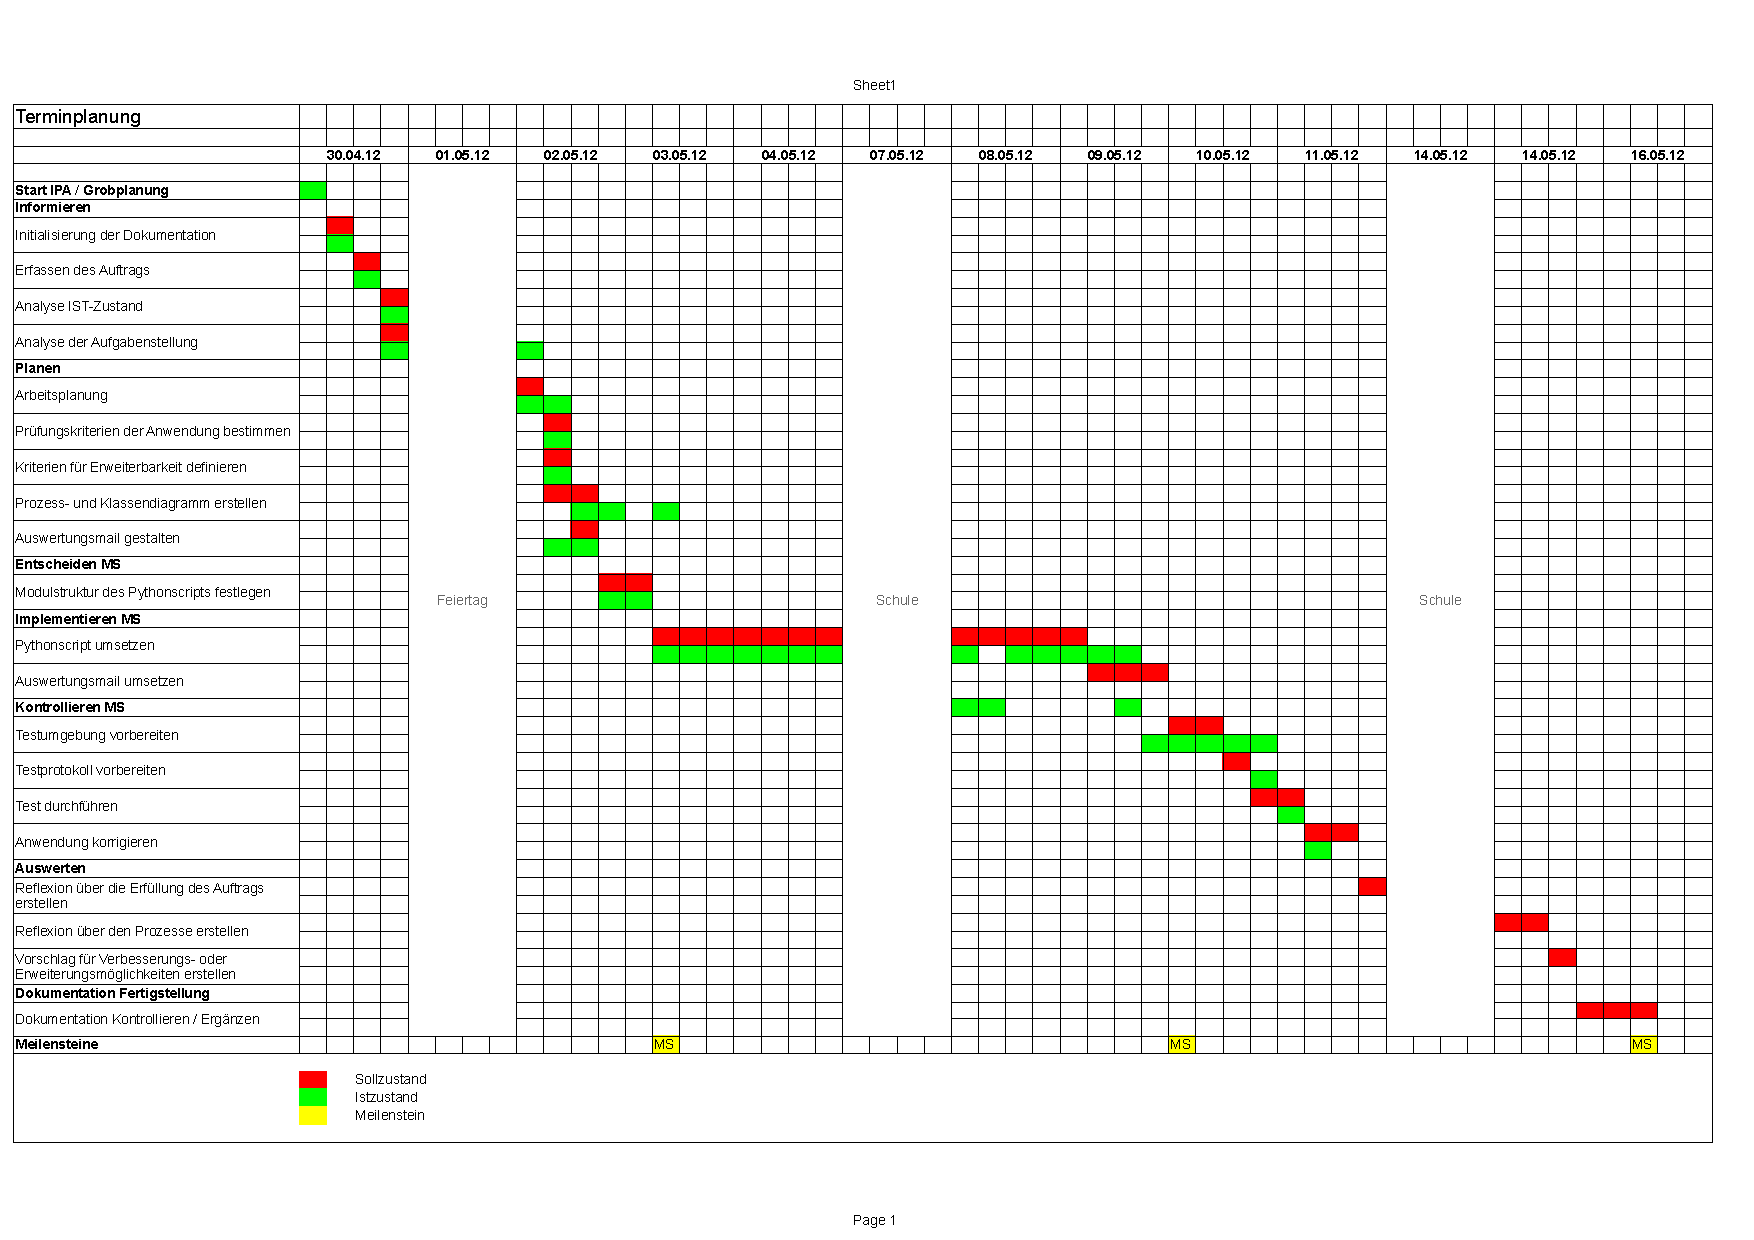
\includegraphics[height=1\textwidth,angle=0]{./grafiken/terminplanung.pdf}
\end{center}

    \part{Projekt}
    \part{Tagesjournal}
         \chapter{Tagesjournal}
            %!TEX root = ../dokumentation.tex

\begin{table}
\section{Reflexion vom 30.4.2012}
\begin{tabular}{| l | p{12cm} |}
    \hline
    Tätigkeiten &
    \begin{itemize}
        \item Initialisierung der Dokumentation 
        \item Erfassen des Auftrags
        \item Analyse des Ist-Zustands
        \item Analyse der Aufgabenstellung
    \end{itemize}  \\
    \hline
    Probleme &
    Es haben sich keine Probleme ergeben. \\
    \hline
    Erreichte Ziele &
    Es wurde alle Ziele ausser der ''Analyse der Aufgabenstellung'' erreicht. Es bin mit der Analyse noch nicht ganz zufrieden. \\
    \hline
    Reflexion &
    Heute habe ich mit meiner IPA begonnen. Ich hatte so gut wie keine Schwirigkeiten zu beginnen. 
    Als erstes habe ich die Dokumentation initialisiert. Das heisst ich habe mir eine Vorlage in Latex zusammengestellt, damit ich mich auf den Inhalt konzentrieren kann und nicht auf das Layout.
    Als nächstes habe ich eine Grobplannung für mein Projekt erstellt. Die detailierte Planung werde ich erst erstellen können, wenn ich die Analyse abgeschlossen habe.
    Mit der Analyse des Ist-Zustands habe ich auch schon begonnen. Bis jetzt bin ich noch auf keine Probleme gestossen. Es sind jediglich ein paar Optimierungsideen bei den ''pre-commit hooks'' aufgetaucht. Diese werde ich noch mit meinem Vorgesetzten besprechen müssen.  
    Um 16.00 bis 16.30 hatte ich mein erstes Gespräch mit meinem Experten. Ich konnte sicher auf seine Fragen antworten, was bestätigt, dass ich die Aufgabenstellung richtig verstanden habe. \\
    \hline
\end{tabular}
\end{table}
\clearpage


            %!TEX root = ../dokumentation.tex
\section{Reflexion vom 2.5.2012}

\begin{table}
\begin{tabular}{| l | p{10cm} |}
    \hline
    Tätigkeiten &
    \begin{itemize}
    \item Arbeitsplanung vervollständigen
    \item Prüfungskriterien bestimmen
    \item Kriterien für die Erweiterbarkeit definieren
    \item Prozessdiagramm erstellen
    \item Prüfungsbericht gestalten
    \item Beginn mit der Definition der Modulstruktur
\end{itemize}  \\
    \hline
    Probleme & 
    Es haben sich keine bemerkenswerte Probleme ergeben. \\
    \hline
    Erreichte Ziele &
    Laut der Terminplanung wurden alle Ziele am heutigen Tag erreicht. \\
    \hline 
    Reflexion &
    Ich habe heute meine ersten Meilenstein erreicht. Es wahr teilweise etwas mühsam so oft zwischen den verschiedenen Arbeiten zu wechseln. Manchmal sind mir wieder Sachen eingefallen, die einen anderen Arbeitsschritt betreffen. Ich kann mir gut vorstellen, dass ich noch im Verlauf der Arbeit wieder zu der Definition der Prüfungskriterien oder zum Gestalten des Prüfungsbericht zurück muss. Trotzdem bin ich bin mit meinem heutigen Fortschritt zufrieden. \\
    \hline
\end{tabular}
\end{table}

\clearpage

    %     \chapter{Realisierung}
    %         \input{./kapitel/05_realisierung.tex}
    %     \chapter{Testing}
    %         \input{./kapitel/06_testing.tex}
    %     \chapter{Konklusion}
    %         \input{./kapitel/07_konklusion.tex}

    
    
    % 
    % \chapter{Abkürzungsverzeichnis}
    %     \input{./kapitel/09_acronym.tex}
    % \lstlistoflistings
  
    
    % \chapter{Literaturverzeichnis}
    %     \input{./kapitel/08_quellen.tex}
    % 
    % \chapter{Arbeitsjournal}
    %     \input{../arbeitsjournal/arbeitsjournal.tex}
    
\end{document}
